\section{INTRODUCCIÓN}
\subsection{Introducción}
En los últimos años, gracias al gran desarrollo tecnológico que se ha vivido tanto a nivel de computo (mejorando la eficiencia y el uso de los recursos disponibles) como a nivel de transmisión de datos (mejorando las comunicaciones), ha permitido a las organizaciones el almacenamiento de una gran cantidad de información.

Para comprender mejor este gran volumen de información, es necesario utilizar métodos, técnicas, herramientas además de personas con conocimientos (formando todas esta un vínculo estrecho) que permita y ayude a explotar, investigar, predecir y obtener información relevante para tomar decisiones de forma adecuada.

\subsection{Contexto}
La organización educativa no ha quedado ajena a estas necesidades de una mejor comprensión de los datos. Desde la Consejería de Educación de Madrid se están realizando proyectos para conseguir sacar la máxima información del gran número de datos que se poseen.

Obviamente, debido a este gran tamaño de datos, es necesario utilizar métodos, herramientas y personas con conocimientos para obtener información concreta en un tiempo legible. Desde la Consejería de Educación se quiere tener conocimientos actuales sobre la situación educativa. Un ejemplo podría ser el número de alumnos matriculados con necesidades educativas para un determinado centro de la Dirección de Área Territorial Sur. No solo eso, también podrían obtenerse alumnos de un determinado nivel educativo o incluso grupos.

%http://www.superiorinfotech.com/bidw.html
\begin{figure*}[htb]
	\centering
	\caption{
		Arquitectura de un almacén de datos. Recuperado de: Superior Information Technology.
	}
	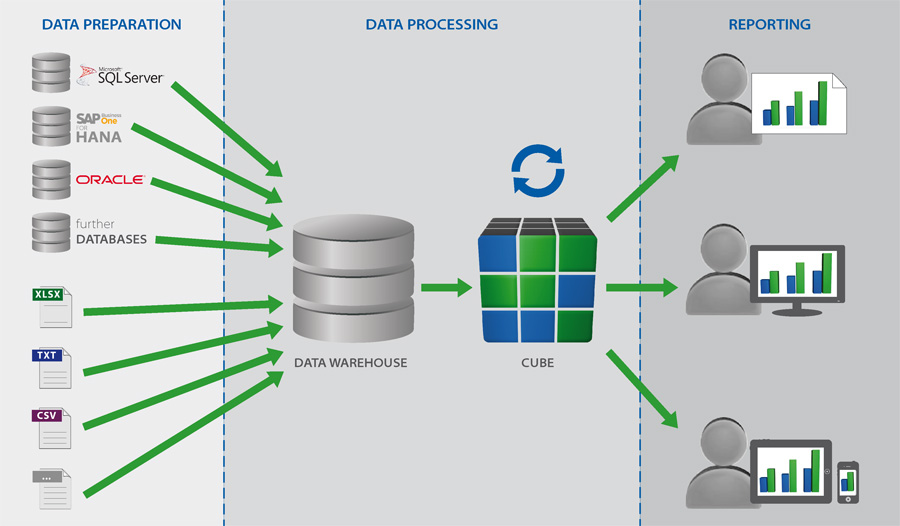
\includegraphics[width=0.6\textwidth]{recursos/arquitecturaDatawarehouse}
	\label{fig:ArqDWH}
\end{figure*}

En la figura \ref{fig:ArqDWH} se pude observar la arquitectura de un almacén de datos. Mediante esta arquitectura, los usuarios finales pueden obtener mucha información sin necesidad de realizar consultas complejas a bases de datos.

No obstante, mostrar la información actual o pasada no es suficiente. La Consejería de Educación también requiere obtener datos futuros. En este aspecto, la Consejería necesita saber cuántos alumnos podrán matricularse en el futuro, con el objetivo de destinar recursos a los centros.
Por tanto, será necesario utilizar técnicas predictivas. Estas técnicas se pueden usar perfectamente en la Consejería puesto que requieren una gran cantidad de datos para realizar pronósticos ajustados, en este sentido, la Consejería tiene un gran histórico de años anteriores.

\subsection{Justificación y Objetivos}
En este sentido (de las predicciones), una unidad de Educación Secundaria Obligatoria de la Consejería de Educación de la Comunidad de Madrid ha planteado un problema.

El problema con el que se enfrenta esta unidad cada día es la planificación de grupos para el siguiente curso. Esta planificación es la base para poder decidir donde se escolariza cada alumno y como se va a repartir la plantilla del profesorado según sus especialidades. Conocer el número de grupos permite, por tanto, un óptimo reparto de la plantilla de docentes y recursos. De esta forma, además, se evita la existencia de grupos sobrepoblados.

Desde esta unidad, se ha informado sobre aspectos con los que trabajan para poder realizar una predicción acerca del número de grupos para curso venidero. 

Estos aspectos son:
\begin{enumerate}
	\item Escolaridad del curso actual.
	\begin{itemize}
		\item Número de alumnos y grupos de un determinado centro.
		\item El número de alumnos por aula (también conocido como ratio).
		\item Matriculación de nuevos alumnos.
		\begin{itemize}
			\item Principalmente alumnos que superan el nivel de 6º de primaria y pasan a 1º de ESO.
		\end{itemize}
	\end{itemize}
	
	\item Bilingüismo del centro. Muchos alumnos optan por centros bilingües para su mejor formación, por lo que estos centros suelen tener más demanda de alumnos.
	\item Posibilidad de creación de nuevas zonas urbanas cerca del centro. 
	\item Posibilidad de apertura o cierre de centros educativos. El cierre, por ejemplo, de un centro privado provocara una mayor tasa de matriculación de los centros contiguos. 
	\item Porcentaje de aprobados. Los alumnos que están ya matriculados tienen prioridad sobre los nuevos alumnos, por lo tanto, si existe una alta tasa de suspensos, quedan pocas plazas de admisión de nueva matricula.
	\item El número y la aparición de nuevas enseñanzas. La oferta de nuevas enseñanzas atraerá a nuevos alumnos al centro, incrementando así el número de matriculaciones.
\end{enumerate}

La unidad actualmente utiliza herramientas manuales para conseguir conocer el número de grupos, indicando que es un trabajo mecánico y con herramientas obsoletas, evitando la posibilidad de inclusión de nuevas variables o factores que impliquen nuevos resultados.

Por ello, con este TFM se propone dar una solución al problema actual mediante el uso de herramientas y métodos flexibles que automaticen dichas tareas y proponga, además, nuevas variables o factores que puedan influir en la toma de decisión. El objetivo final consiste, por tanto, en obtener predicciones precisas para la toma de decisiones. 

Los objetivos que se quiere cumplir con este TFM son los siguientes:
\begin{itemize}
	\item Seleccionar variables que interesen estudiar y que aporten valor en el desarrollo de este TFM.
	\item Obtener modelos que se ajusten correctamente a los datos y que aporten una gran precisión.
	\item Realizar predicciones con datos existentes.
\end{itemize}

\subsection{Metodología}

Para ello, en primer lugar, se van a realizar reuniones con los responsables de la unidad de Educación Secundaria. A partir de estas reuniones se van a obtener las fuentes donde se encuentre la información relevante. Una vez que se conocen las fuentes, se van a estructura los datos existentes.

Después se seleccionarán aquellos datos que se consideran importantes para realizar las labores de predicción. Para realizar la selección, se debe estudiar los mecanismos ya existentes en esta Unidad de Secundaria para obtener aquellos en uso. Una vez que se han seleccionado los datos, se va a realizar un tratamiento de estos para poder utilizarlos en las nuevas herramientas.

Por último, se van a aplicar modelos predictivos y se van a seleccionar aquellos que mayor precisión aporten con dichos datos.

\subsection{Organización del TFM}
La estructura que se va a seguir en el TFM va a ser la siguiente:
\begin{itemize}
	\item \textbf{Capitulo 1. Introducción:} En el primer capítulo se van a definir las necesidades existentes que justifican el desarrollo de este trabajo. También se va a definir los objetivos que se persiguen con la realización de este. Por último, se presenta la estructura que tendrá el presente documento.
	\item \textbf{Capitulo 2. Justificación teórica:} En este segundo capítulo se va a realizar una investigación sobre el estado de la cuestión. Se va a realizar un estudio sobre los métodos, modelos y usos de la minería de datos en el ámbito educativo. 
	\item \textbf{Capitulo 3. Propuesta de intervención:} En este tercer capítulo se va a plantear una solución al problema existente. 
	\item \textbf{Capitulo 4. Diseño de la investigación:} Este capítulo va a definir los pasos que se seguirán en la realización de un proyecto de minería de datos. Se van a detallar también las tareas que se van a desempeñar en cada uno de los pasos.
	\item \textbf{Capitulo 5. Conclusiones:} En este capítulo se van a detallar las conclusiones obtenidas a partir de los resultados alcanzados.
\end{itemize}





